\UC{Visualizzazione riepilogo ordini in gestione}
\label{visualizzazione-ordini-in-gestione}

Il venditore vuole vedere gli ordini chiusi o da gestire.
\begin{itemize}
    \item \textbf{Attori primari:} venditore;
    \item \textbf{Precondizione:} il venditore da qualsiasi schermata in cui si trovi vuole visualizzare gli ordini da gestire o già chiusi;
    \item \textbf{Postcondizione:} il venditore vede tutti gli ordini a suo carico in ordine cronologico decrescente;
    \item \textbf{Scenario principale:} il venditore vuole vedere tutti gli ordini a suo carico da gestire o già chiusi ed accede alla schermata di riepilogo ordini. Il venditore seleziona la funzionalità per accedere all'elenco degli ordini effettuati sulla piattaforma e visualizza l'elenco degli ordini ricevuti sulla piattaforma, dove è indicato per ogni ordine:
    \begin{itemize}
    	\item Il codice dell'ordine;
    	\item Lo stato dell'ordine;
    	\item Il prezzo totale che è stato pagato;
    	\item L'indirizzo a cui è stato consegnato o verrà consegnato;
    	\item L'indirizzo e-mail dell'acquirente che ha effettuato l'ordine;
    	\item Una lista di tutti i prodotti acquistati in quell'ordine, dove per ogni prodotto verrà visualizzato:
    	\begin{itemize}
    		\item Nome del prodotto;
    		\item Quantità acquistata;
    		\item Prezzo totale del prodotto a cui è stato acquistato.
    	\end{itemize}
    \end{itemize}
	\item \textbf{Scenari alternativi:} 
	\begin{enumerate}[label=\lett]
		\item Il venditore non ha ancora ricevuto ordini, viene visualizzato il messaggio "Nessun ordine ricevuto" e viene data la possibilità al venditore di tornare alla propria dashboard.
	\end{enumerate}
\end{itemize}

\UC{Modifica stato ordine}
\label{modifica-stato-ordine}

Il venditore vuole modificare lo stato di un determinato ordine.
\begin{itemize}
	\item \textbf{Attori primari:} venditore;
	\item \textbf{Precondizione:} il venditore ha intenzione di modificare lo stato di un ordine a suo carico;
	\item \textbf{Postcondizione:} il venditore ha modificato lo stato di un ordine;
	\item \textbf{Scenario principale:}
	\begin{itemize}
		\item Il venditore seleziona un ordine dalla lista;
		\item Il venditore modifica lo stato dell'ordine.
	\end{itemize}
\end{itemize}

\UC{Ricerca di un ordine per codice}
\label{ricerca-codice-ordine-venditore}

Il venditore può cercare un ordine dalla propria schermata di riepilogo ordini.
\begin{itemize}
	\item \textbf{Attori primari:} venditore;
	\item \textbf{Precondizione:} il venditore ha selezionato la funzionalità per la ricerca e l'inserimento del codice per individuare un ordine;
	\item \textbf{Postcondizione:} il venditore visualizza l'ordine che corrisponde al codice per il quale si è svolta la ricerca;
	\item \textbf{Scenario principale:} il venditore ha selezionato la funzione prevista per la ricerca. Dopo aver inserito il codice per individuare l'ordine, conferma la ricerca e viene aggiornata la schermata di riepilogo ordini che mostra solamente l'ordine corrispondente al codice indicato;
	\item \textbf{Scenari alternativi:}
	\begin{enumerate}[label=\lett]
		\item Il venditore ha svolto una ricerca che non ha trovato coincidenze con nessun ordine ricevuto. In questo caso la schermata di riepilogo ordini viene aggiornata mostrando il messaggio nessun ordine trovato.
	\end{enumerate}
 \item \textbf{Estensioni:}
\begin{enumerate}[label=\lett]
	\item Il venditore inserisce un codice che non rispetta il formato standard uuid v4. In questo caso:
	\begin{itemize}
		\item (UC\ref{estensione:codice-ordine-non-valido}) - Verrà visualizzato il messaggio d'errore codice dell'ordine non valido;
		\item Non verrà eseguita la ricerca.
	\end{itemize}
\end{enumerate}
\end{itemize}

\UC{Ricerca di un ordine per cliente}
\label{ricerca-cliente-ordine-venditore}

Il venditore può cercare gli ordini in base al cliente che lo ha effettuato.
\begin{itemize}
	\item \textbf{Attori primari:} venditore;
	\item \textbf{Precondizione:} il venditore è nella schermata di riepilogo ordine ed ha inserito l'indirizzo e-mail di uno uno tra i clienti che hanno effettuato un ordine a suo carico;
	\item \textbf{Postcondizione:} il venditore visualizza la lista di ordini effettuati dal cliente per il quale si è svolta la ricerca;
	\item \textbf{Scenario principale:} il venditore ha selezionato la funzione prevista per la ricerca. Dopo aver inserito il cliente per individuare gli ordini, conferma la ricerca e viene aggiornata la schermata di riepilogo ordini che mostra solamente gli ordini effettuati dal cliente indicato;
	\item \textbf{Scenari alternativi:}
	\begin{enumerate}[label=\lett]
		\item Il venditore ha svolto una ricerca che non ha trovato coincidenze con nessun cliente. In questo caso la schermata di riepilogo ordini viene aggiornata mostrando il messaggio nessun ordine trovato.
	\end{enumerate}
\end{itemize}

\UC{Filtraggio ordini nella schermata di riepilogo ordini}
\label{filtro-ordini-venditore}

\begin{figure}[H]
    \centering
    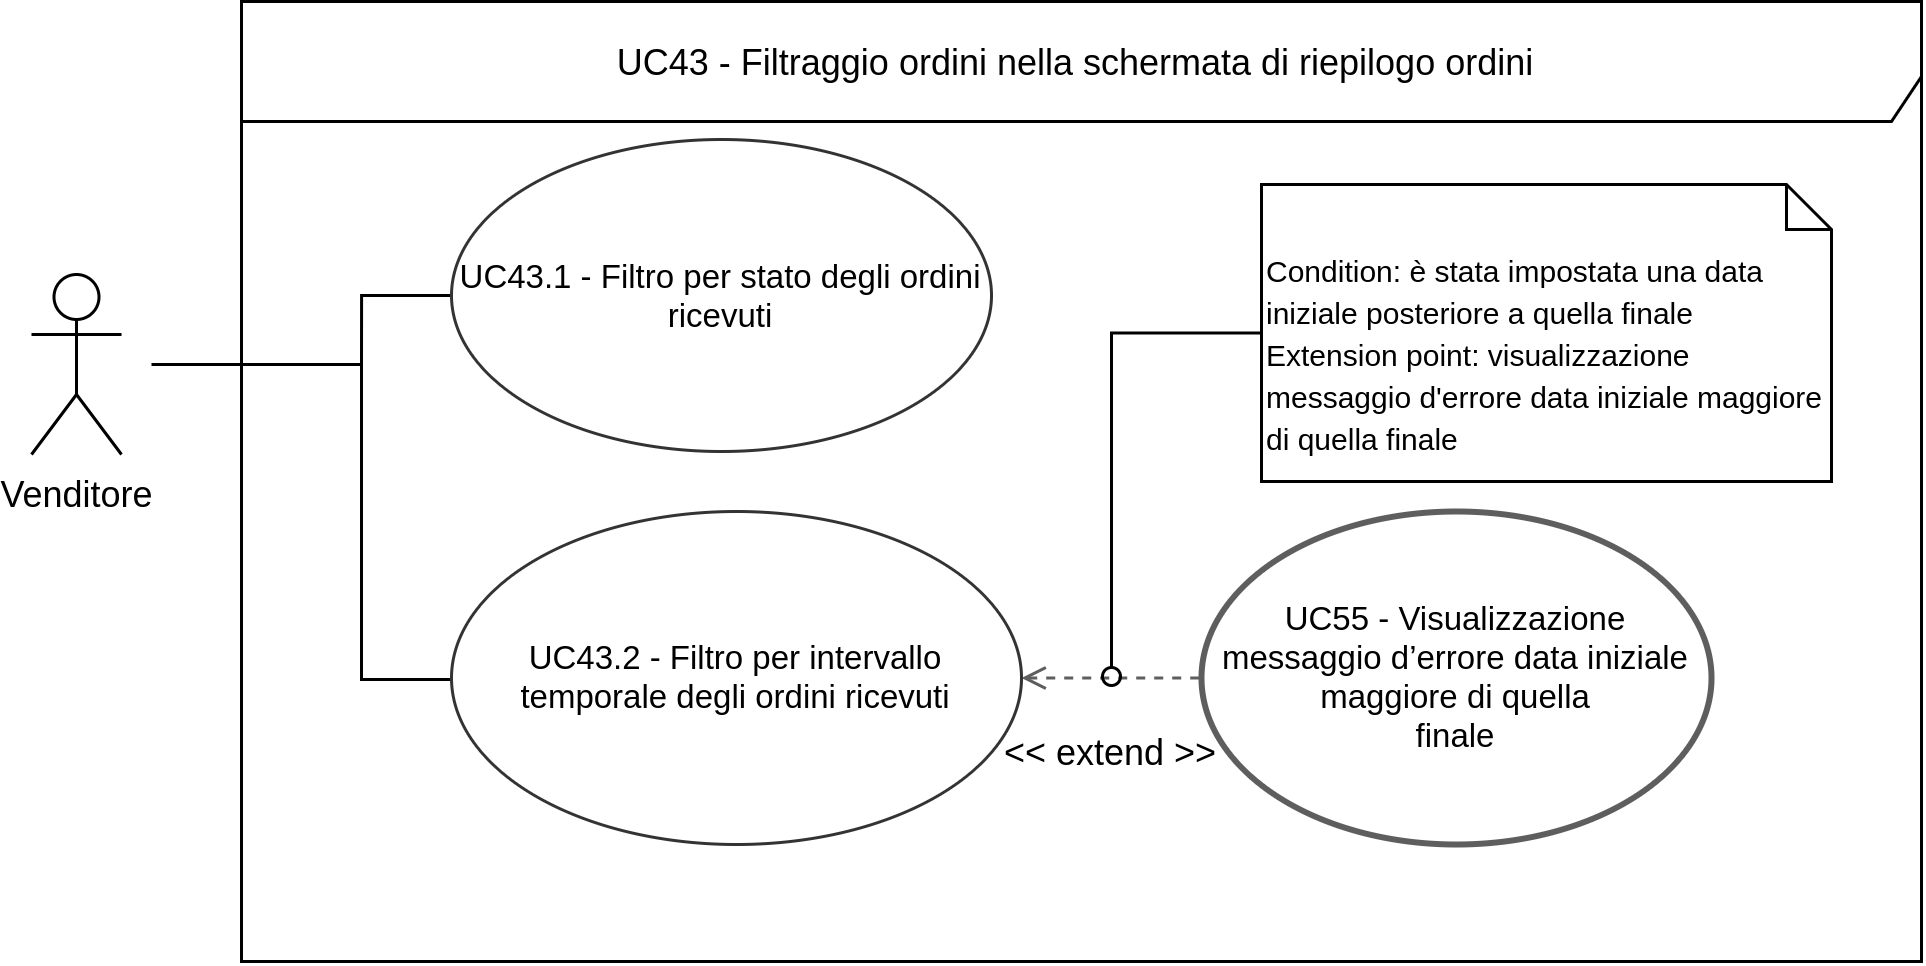
\includegraphics[width=\textwidth]{Immagini/DiagrammiUC/Venditore/FiltraggioOrdiniVenditore.png}
    \caption{Diagramma di \actualUC: Filtraggio ordini nella schermata di riepilogo ordini}
    \label{fig:filtro-ordini-venditore}
\end{figure}

Il venditore può filtrare gli ordini nella schermata di riepilogo ordini per lo stato dell'ordine secondo un intervallo temporale ed ordinarli in base alla loro data di accettazione.
\begin{itemize}
	\item \textbf{Attori primari:} venditore;
	\item \textbf{Precondizione:} il venditore è nella schermata di riepilogo ordini e ha impostato uno (o più) dei filtri disponibili per i quali cercare;
	\item \textbf{Postcondizione:} il venditore avrà a disposizione tutti gli ordini che soddisfano tutte le condizioni dei vari filtri impostati;
	\item \textbf{Scenario principale:} l'attore è nella schermata di riepilogo ordini e ha impostato uno (o più) dei seguenti filtri:
	\begin{itemize}
		\item (UC\ref{filtro-ordini-venditore.stato}) - Impostazione del filtro per stato degli ordini ricevuti;
		\item (UC\ref{filtro-ordini-venditore.temporale}) - Impostazione del filtro per intervallo temporale degli ordini ricevuti.
	\end{itemize}
	Di seguito la schermata di riepilogo ordini verrà aggiornata con gli ordini che rispettano tutti i filtri applicati;
	\item \textbf{Scenari alternativi:}
	\begin{enumerate}[label=\lett]
		\item Il venditore ha impostato i filtri in modo tale che la ricerca con la loro combinazione non dia alcun risultato. In questo caso la schermata di riepilogo ordini viene aggiornata mostrando il messaggio nessun ordine trovato.
	\end{enumerate}
\end{itemize}

\subUC{Filtro per stato degli ordini ricevuti}
\label{filtro-ordini-venditore.stato}

Il venditore può cercare gli ordini in base al loro stato, selezionando quelle di interesse tra tutti quelli disponibili.
\begin{itemize}
	\item \textbf{Attori primari:} venditore;
	\item \textbf{Precondizione:} il venditore è nella schermata di riepilogo ordini e ha selezionato uno (o più) stati tra quelli disponibili per quali filtrare;
	\item \textbf{Postcondizione:} il venditore visualizzerà nella schermata di riepilogo ordini gli ordini a suo carico che si trovano in uno degli stati selezionati;
	\item \textbf{Scenario principale:} il venditore è nella schermata di riepilogo ordini e ha selezionato uno (o più) stati tra quelli disponibili per quali filtrare e di seguito verranno visualizzati gli ordini che appartengono ad almeno uno degli stati selezionati;
	\item \textbf{Scenari alternativi:}
	\begin{enumerate}[label=\lett]
		\item Se il venditore non imposta il seguente filtro, allora verranno visualizzati tutti gli ordini ricevuti.
	\end{enumerate}
\end{itemize}

\subUC{Filtro per intervallo temporale degli ordini ricevuti}
\label{filtro-ordini-venditore.temporale}

\begin{figure}[H]
    \centering
    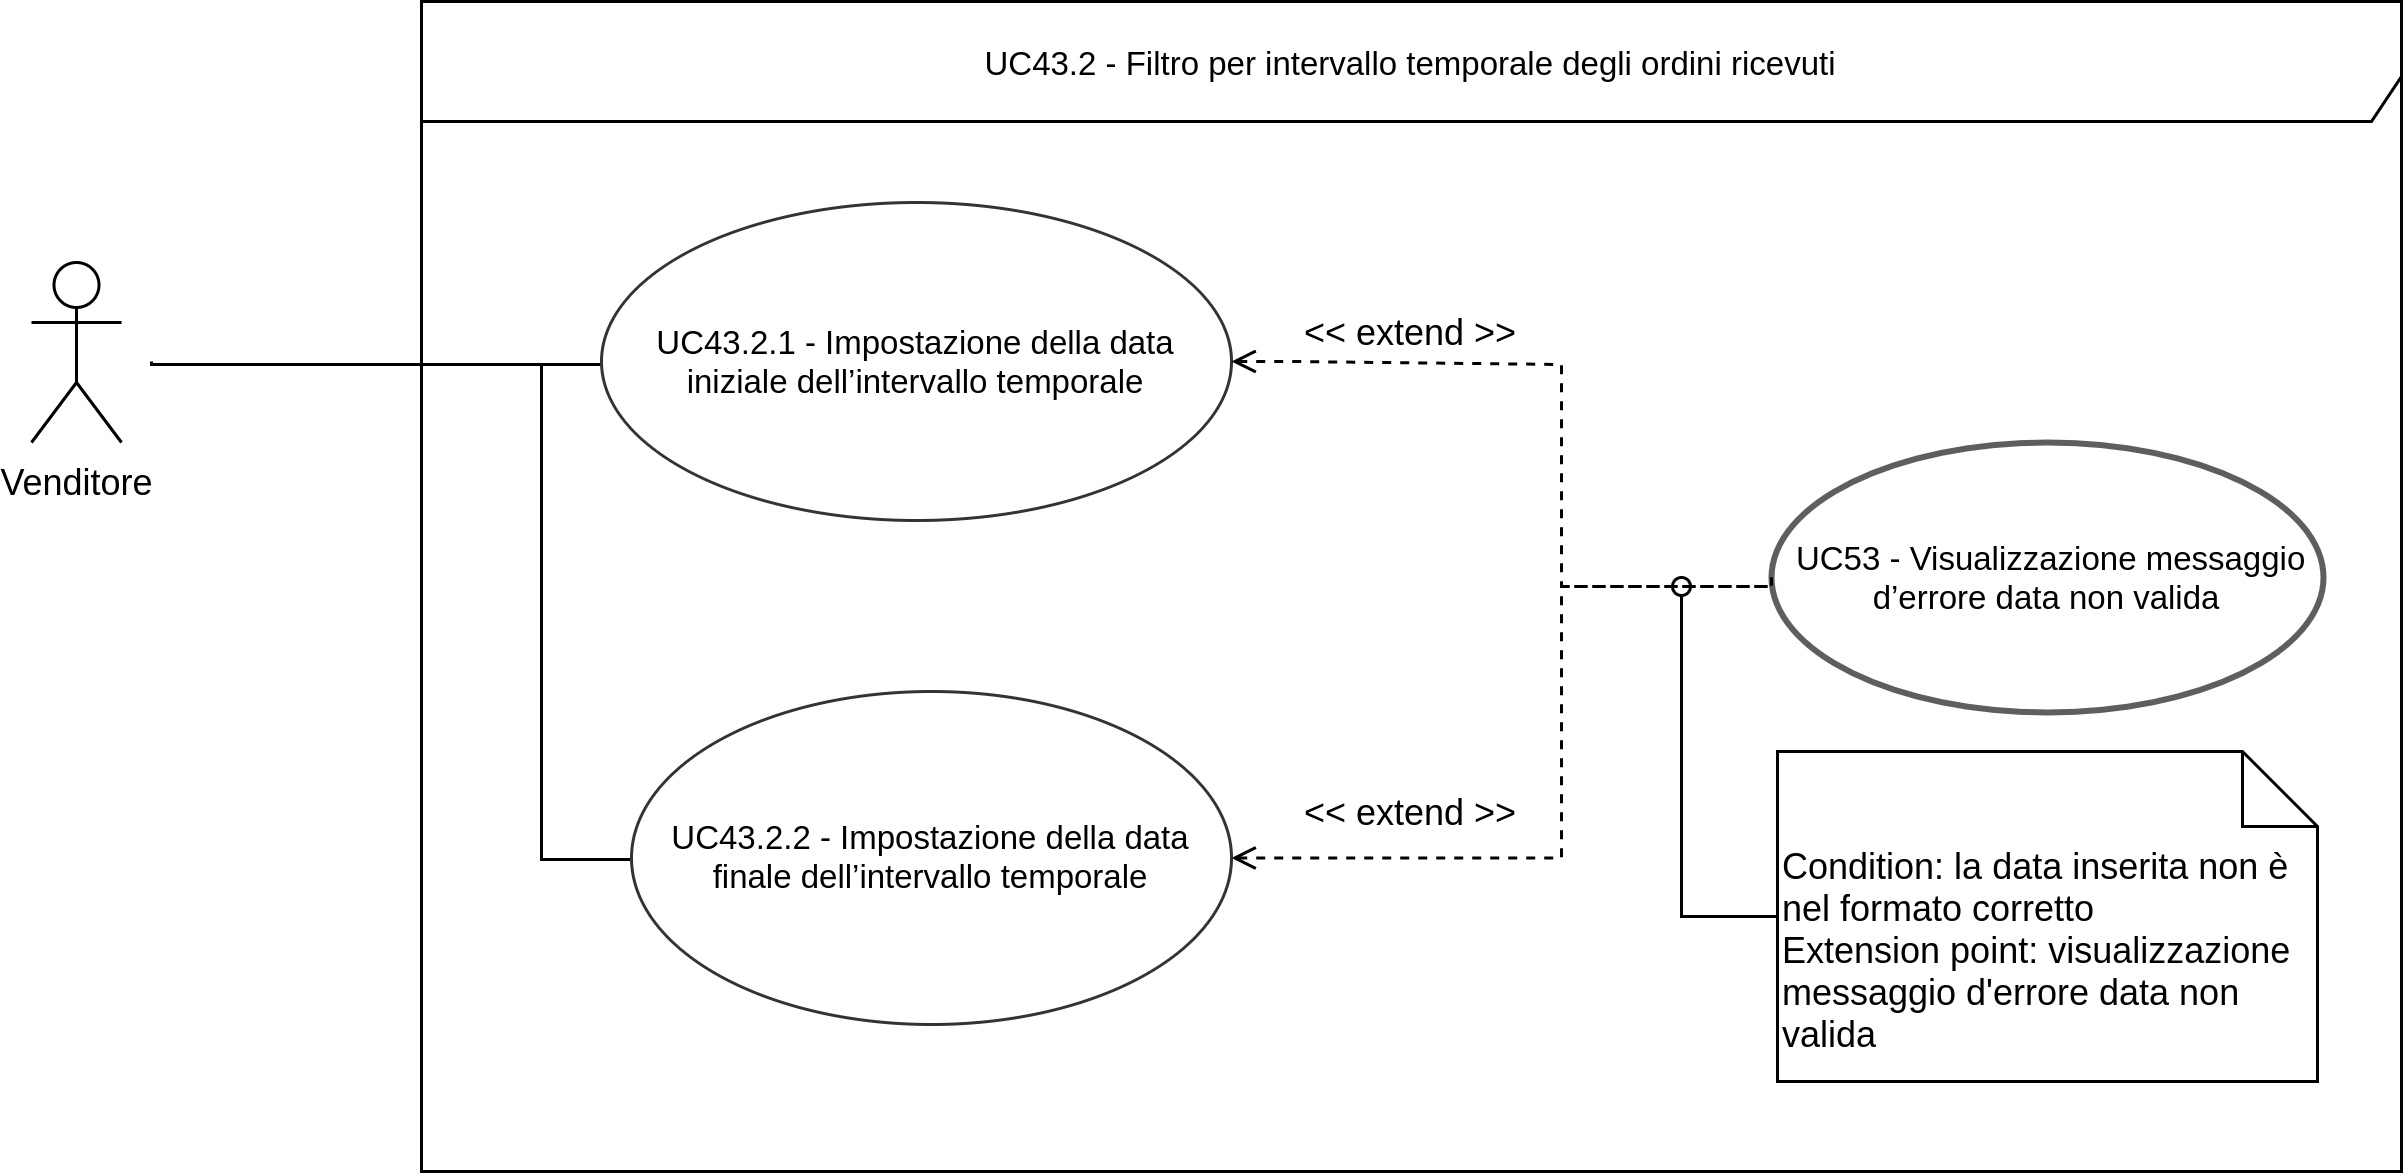
\includegraphics[width=\textwidth]{Immagini/DiagrammiUC/Venditore/FiltroIntervalloTemporaleVenditore.png}
    \caption{Diagramma di \actualSubUC: Filtro per intervallo temporale degli ordini ricevuti}
    \label{fig:filtro-ordini-venditore.temporale}
\end{figure}

Il venditore filtra temporalmente l'elenco degli ordini a suo carico sulla piattaforma.
\begin{itemize}
	\item \textbf{Attori primari:} venditore;
	\item \textbf{Precondizione:} il venditore si trova nella schermata di riepilogo ordini;
	\item \textbf{Postcondizione:} il venditore visualizza tutti gli ordini che sono stati fatti tra la data di inizio e quella di fine impostate;
	\item \textbf{Scenario principale:} il venditore si trova nella schermata di riepilogo ordini e vuole filtrare gli ordini a suo carico ricevuti durante un certo intervallo temporale. Per farlo dovrà:
	\begin{itemize}
		\item (UC\ref{filtro-ordini-venditore.temporale.data-iniziale}) - Impostare la data iniziale dell'intervallo temporale;
		\item (UC\ref{filtro-ordini-venditore.temporale.data-finale}) - Impostare la data finale dell'intervallo temporale.
	\end{itemize}
		\item \textbf{Scenari alternativi:}
	\begin{enumerate}[label=\lett]
		\item Se il venditore non imposta il seguente filtro, allora verranno visualizzati tutti gli ordini ricevuti dal più al meno recente.
	\end{enumerate}
	\item \textbf{Estensioni:}
	\begin{enumerate}[label=\lett]
		\item Il venditore inserisce una data iniziale maggiore di quella finale. In questo caso:
		\begin{itemize}
			\item (UC\ref{estensione:data-iniziale-maggiore-data-finale}) - Viene visualizzato il messaggio d'errore data iniziale maggiore di quella finale;
			\item Non verrà eseguita la ricerca.
		\end{itemize}
	\end{enumerate}
\end{itemize}

\subSubUC{Impostazione della data iniziale dell'intervallo temporale}
\label{filtro-ordini-venditore.temporale.data-iniziale}

Il venditore imposta la data iniziale dell'intervallo per il quale filtrare l'elenco degli ordini a suo carico ricevuti sulla piattaforma.
\begin{itemize}
	\item \textbf{Attori primari:} venditore;
	\item \textbf{Precondizione:} il venditore si trova nella schermata di riepilogo ordini;
	\item \textbf{Postcondizione:} il venditore ha impostato la data iniziale dell'intervallo per la quale filtrare l'elenco degli ordini ricevuti sulla piattaforma;
	\item \textbf{Scenario principale:} il venditore inserisce una data valida e minore o uguale a quella finale, come data iniziale dell'intervallo per la quale filtrare l'elenco degli ordini ricevuti;
	\item \textbf{Estensioni:}
	\begin{enumerate}[label=\lett]
		\item Il venditore inserisce una data iniziale non nel formato corretto. In questo caso:
		\begin{itemize}
			\item (UC\ref{estensione:data-non-valida}) - Viene visualizzato il messaggio d'errore data non valida;
			\item Non verrà eseguita la ricerca.
		\end{itemize} 
	\end{enumerate}
\end{itemize}

\subSubUC{Impostazione della data finale dell'intervallo temporale}
\label{filtro-ordini-venditore.temporale.data-finale}

Il venditore imposta la data finale dell'intervallo per il quale filtrare l'elenco degli ordini a suo carico ricevuti sulla piattaforma.
\begin{itemize}
	\item \textbf{Attori primari:} venditore;
	\item \textbf{Precondizione:} il venditore si trova nella schermata di riepilogo ordini;
	\item \textbf{Postcondizione:} il venditore ha impostato la data finale dell'intervallo per la quale filtrare l'elenco degli ordini ricevuti sulla piattaforma;
	\item \textbf{Scenario principale:} il venditore inserisce una data valida e maggiore o uguale di quella iniziale, come data finale dell'intervallo per la quale filtrare l'elenco degli ordini ricevuti;
	\item \textbf{Estensioni:}
	\begin{enumerate}[label=\lett]
		\item Il venditore inserisce una data finale non nel formato corretto. In questo caso:
		\begin{itemize}
			\item (UC\ref{estensione:data-non-valida}) - Viene visualizzato il messaggio d'errore data non valida;
			\item Non verrà eseguita la ricerca.
		\end{itemize}
	\end{enumerate}
\end{itemize}